%!TEX root = ../dissertation.tex

\chapter{The Algorithm} \label{cha:algorithm}

%%The purpose of this project is to show how a proto-AGI system such as OpenCog can be used 
Having defined the OpenCog system and part of the implementation of the problem in the previous chapters, it is now possible to combine all the various modules and explain the functioning of the internal design and the main algorithm. \\

It is possible to divide the entire project into 6 phases: initial, perception, learning, request, search and results execution.  

\section{Initial Phase}\label{sec:init}

The initial phase concerns the initialisation of the simulated environment. The framework used for the development and programming of the robot is the well-known ROS, Melodic version, and the Gazebo 9 system handles the simulation. \\
Therefore, the world as in Figure \ref{fig:env_2_named} is loaded into Gazebo. 
It consists of a robot manipulator, some fixed objects  (such as tables, shelves, etc.) and cubes, both with their AprilTags used for detection and semantic assignment. \\
Then, a server in C++ code is activated and the nodes of the ROS system for robot control and object perception become available for listening. \\
Finally, the main AtomSpace is created. 

\begin{figure} [h]
\centering
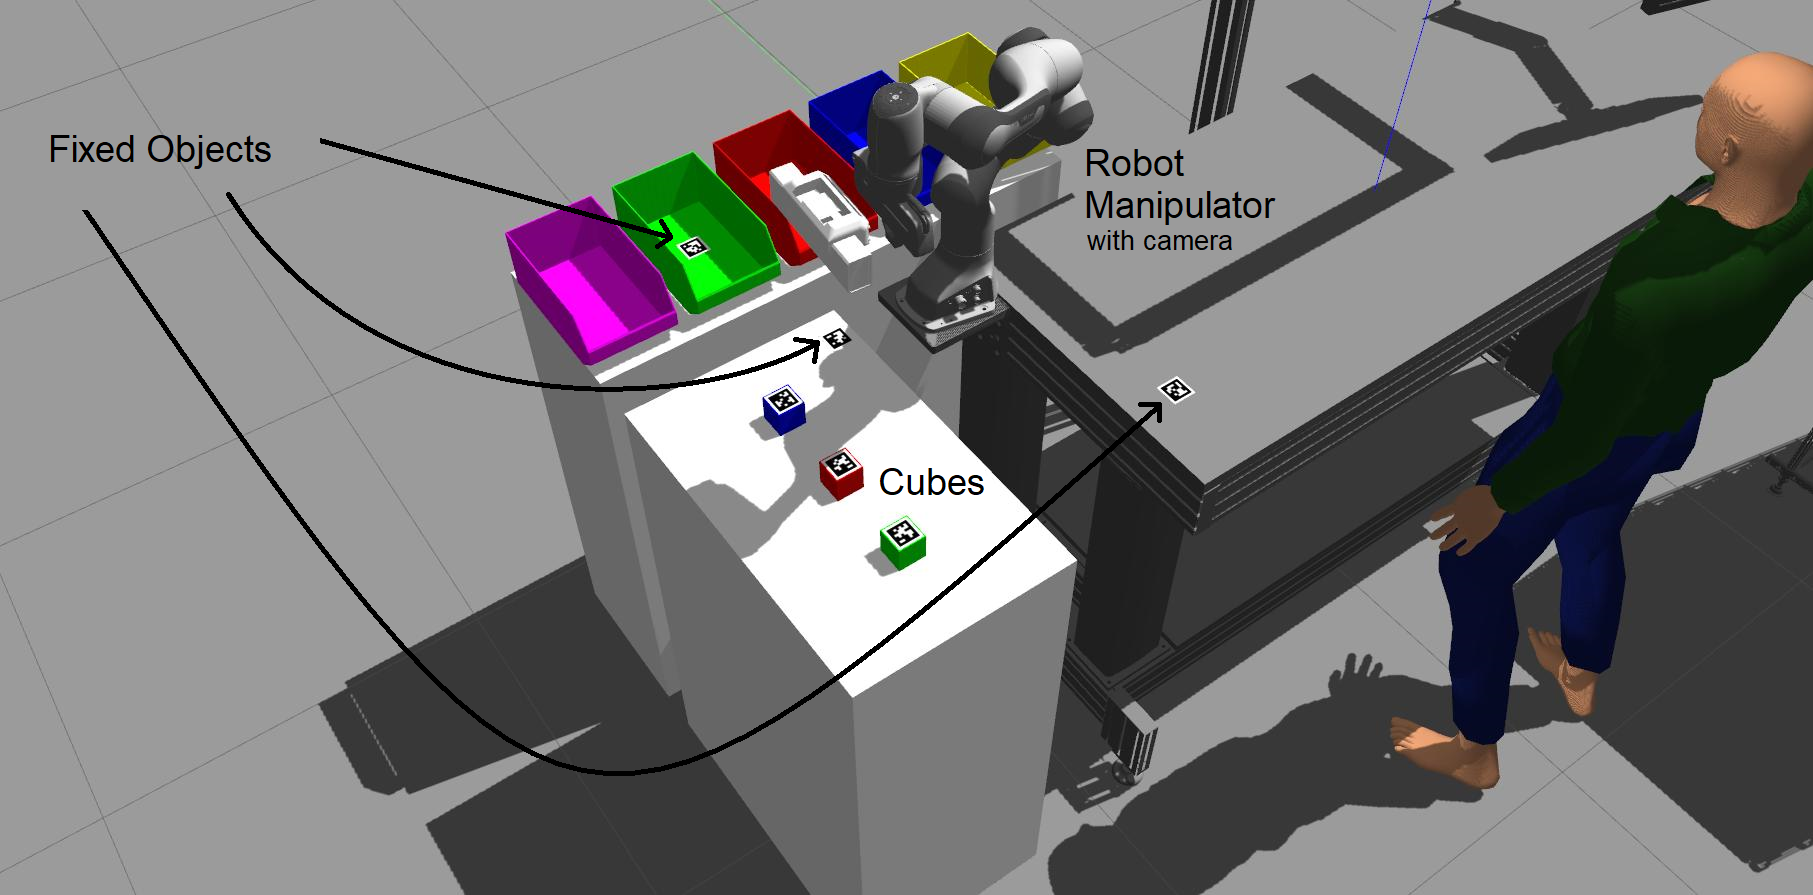
\includegraphics[width=0.9
\textwidth]{figures/Magistrale/env_2_named}
\caption[Environment Components]{ TODO: descrizione
\label{fig:env_2_named}}
\end{figure} 

\section{Perception Phase}\label{sec:perception}

The perception phase, like the remaining phases, is written in Python code and sends commands via a Python client to the C++ server mentioned above. These commands move the robot and allow it to scan its surroundings area for possible objects (related AprilTags are recognised), thanks to the camera attached to the top of it. \\
Of each AprilTag found, its associated semantic representation (i.e. English word describing the object, as well as the name of its relative ConceptNode) is returned by the server to the client, which in turn returns it to the main Python code that begins the initialization of the objects list present in the environment.

\section{Learning Phase}\label{sec:learning}


\section{Request Phase}\label{sec:request}


\section{Search Phase}\label{sec:search}


\section{Results Execution Phase}\label{sec:results_exec}